%%%%%%%%%%%%%%%%%%%%%%%%%%%%%%%%%%%%%%%%%
% Beamer Presentation
% LaTeX Template
% Version 1.0 (10/11/12)
%
% This template has been downloaded from:
% http://www.LaTeXTemplates.com
%
% License:
% CC BY-NC-SA 3.0 (http://creativecommons.org/licenses/by-nc-sa/3.0/)
%
%%%%%%%%%%%%%%%%%%%%%%%%%%%%%%%%%%%%%%%%%

\documentclass[t,usenames,dvipsnames]{beamer}
\mode<presentation> {
\usetheme{Boadilla}
\setbeamertemplate{navigation symbols}{} % To remove the navigation symbols from the bottom of all slides uncomment this line
}

\usepackage{graphicx} % Allows including images
\usepackage{booktabs} % Allows the use of \toprule, \midrule and \bottomrule in tables
\usepackage{amsmath}
\usepackage{amsthm}
\usepackage{cancel}
\usepackage{bussproofs}
\usepackage{proof}
\usepackage{tikz}
\usepackage{wasysym}

\newcommand{\thickarrow}{\raisebox{.5ex}{\tikz \draw[->, line width=.5mm] (0,0) -- (.5,0);}}

\newcommand{\cplanar}{\mathcal{C}_{\operatorname{Planar}}}

\title[Graph minors]{Graph minors\\Robertson and Seymour's theorem in parameterized complexity}

\author{Narek Bojikian} % Your name
\institute[hu-berlin] % Your institution as it will appear on the bottom of every slide, may be shorthand to save space
{
Humboldt University of Berlin\\ % Your institution for the title page
\medskip
\textit{bojikian@informatik.hu-berlin.de} % Your email address
}
\date{\today} % Date, can be changed to a custom date

\begin{document}

\begin{frame}
\titlepage % Print the title page as the first slide
\end{frame}
\begin{frame} \frametitle{Graph minors}
	\begin{minipage}[t]{.59\linewidth}
	\begin{itemize}[<+->]
		\item Given graph $G$.
		\item $H$ is a minor of $G$,
			\begin{itemize}
				\item[] if $H$ results from $G$ by\\
					vertex/edge deletions and \textbf{contractions}.
			\end{itemize}
	\end{itemize}
	\end{minipage}
	\begin{minipage}[t]{.39\linewidth}
			\uncover<4->{Edge-contractions\\}%
			\only<4>{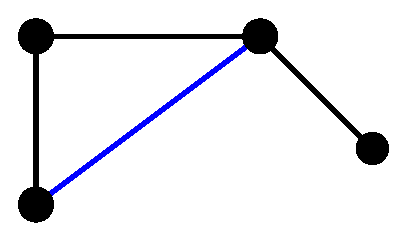
\includegraphics[width=0.9\linewidth]{contraction-0.eps}}%
			\only<5->{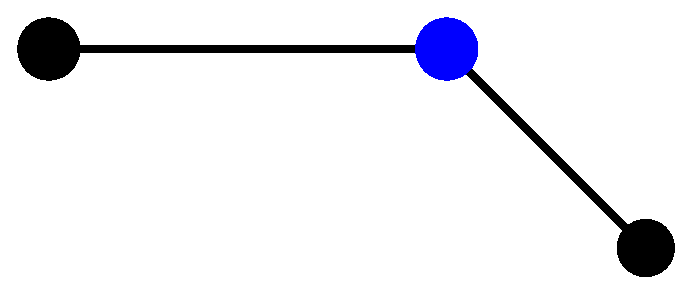
\includegraphics[width=0.9\linewidth]{contraction.eps}}%
	\end{minipage}
	\begin{itemize}[<+->]
		\item []
		\item []
		\item A graph $H$ is a minor of $G$ i.e. ``$H\leq_m G$'' iff\\
			there exists vertex-set $V_h$ f.a. $h \in V(h)$ s.t.
			\begin{itemize}
				\item $G[V_h]$ is connected,
				\item for $g \neq h$ it holds $V_g \cap V_h = \emptyset$,
				\item for $\{g,h\} \in E(H)$, there exist $u_g \in V_g, u_h
					\in V_h$,\\
					s.t. $\{u_g, u_h\} \in E(G)$.
			\end{itemize}
	\end{itemize}
\end{frame}

\begin{frame}\frametitle{Graph minors}
		\begin{itemize}
			\item $G[V_h]$ is connected.
			\item For $g \neq h$ it holds $V_g \cap V_h = \emptyset$.
			\item For $\{g,h\} \in E(H)$, there exist $u_g \in V_g, u_h
				\in V_h$,\\
				s.t. $\{u_g, u_h\} \in E(G)$.
		\end{itemize}
		\vspace{.2cm}
	\uncover<2->{
	\begin{minipage}[t]{.49\linewidth}
			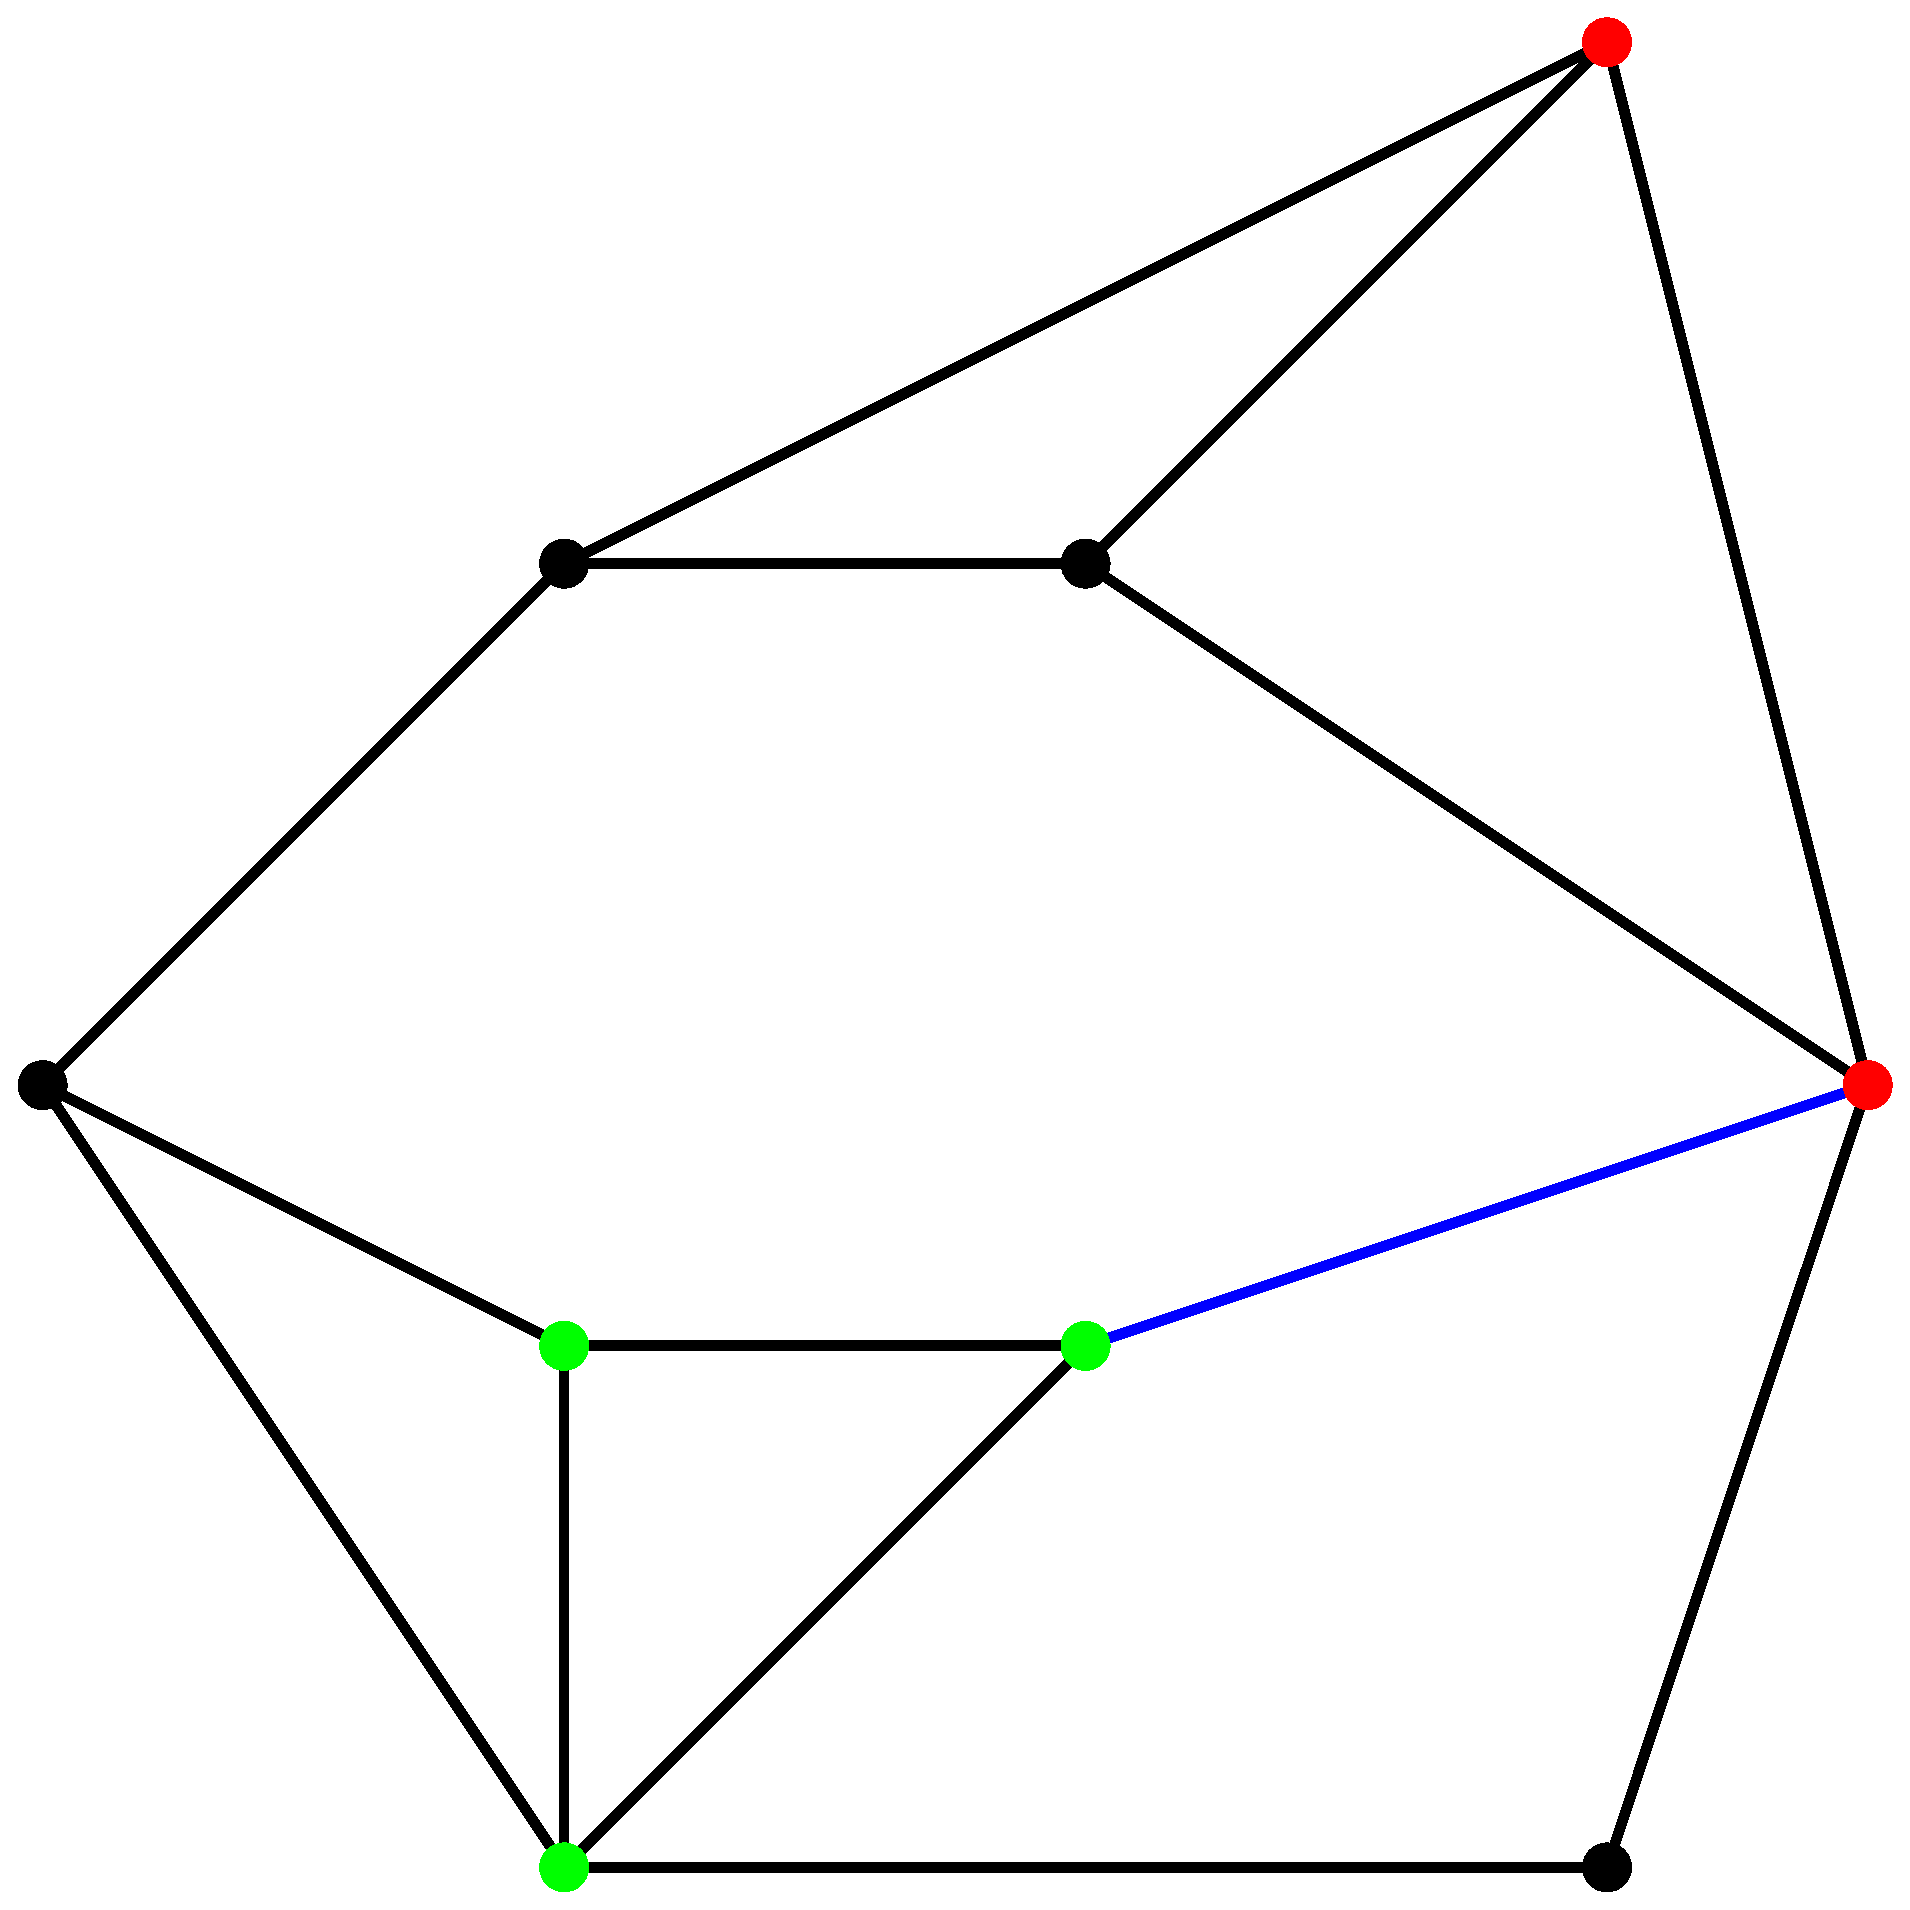
\includegraphics[width=0.8\linewidth]{minor1.eps}%
	\end{minipage}
	\hfill
	\begin{minipage}[t]{.49\linewidth}
			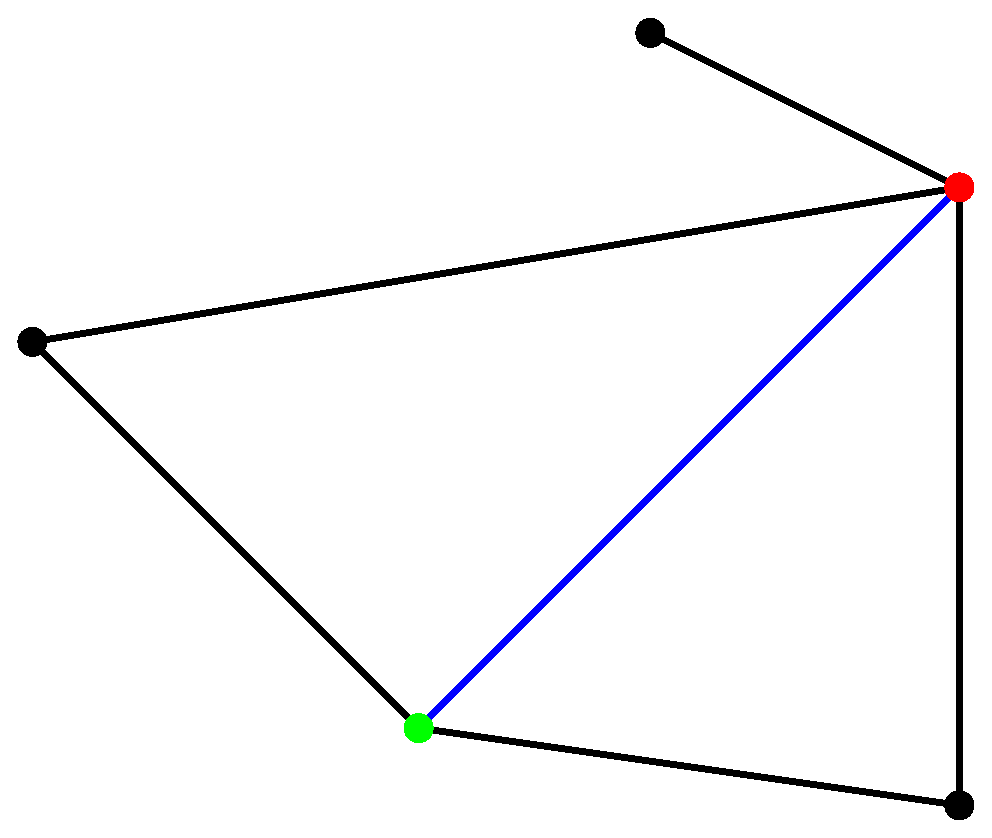
\includegraphics[width=0.8\linewidth]{minor2.eps}%
	\end{minipage}}
	\uncover<3->{
	\thickarrow\hspace{.1cm} Why are both definitions equivalent?}
\end{frame}

\begin{frame} \frametitle{Minor-closed classes}
	\begin{itemize}[<+->]
		\item Let $\mathcal{C}$ be some class of graphs.
		\item We call $\mathcal{C}$ minor-closed, if for all $G \in
			\mathcal{C}$\\
			\hspace{1cm}and $H\leq_m G$ it holds $H \in \mathcal{C}$.
			\\ \vspace{1cm}
	\end{itemize}
	\begin{minipage}{.49\linewidth}
	Examples:
	\begin{itemize}[<+->]
			\item Forests.
			\item Vertex cover number $\leq k$.
			\item \textbf{Planar graphs}.
		\end{itemize}
	\end{minipage}
	\begin{minipage}{.49\linewidth}
		\centering
		\uncover<4->{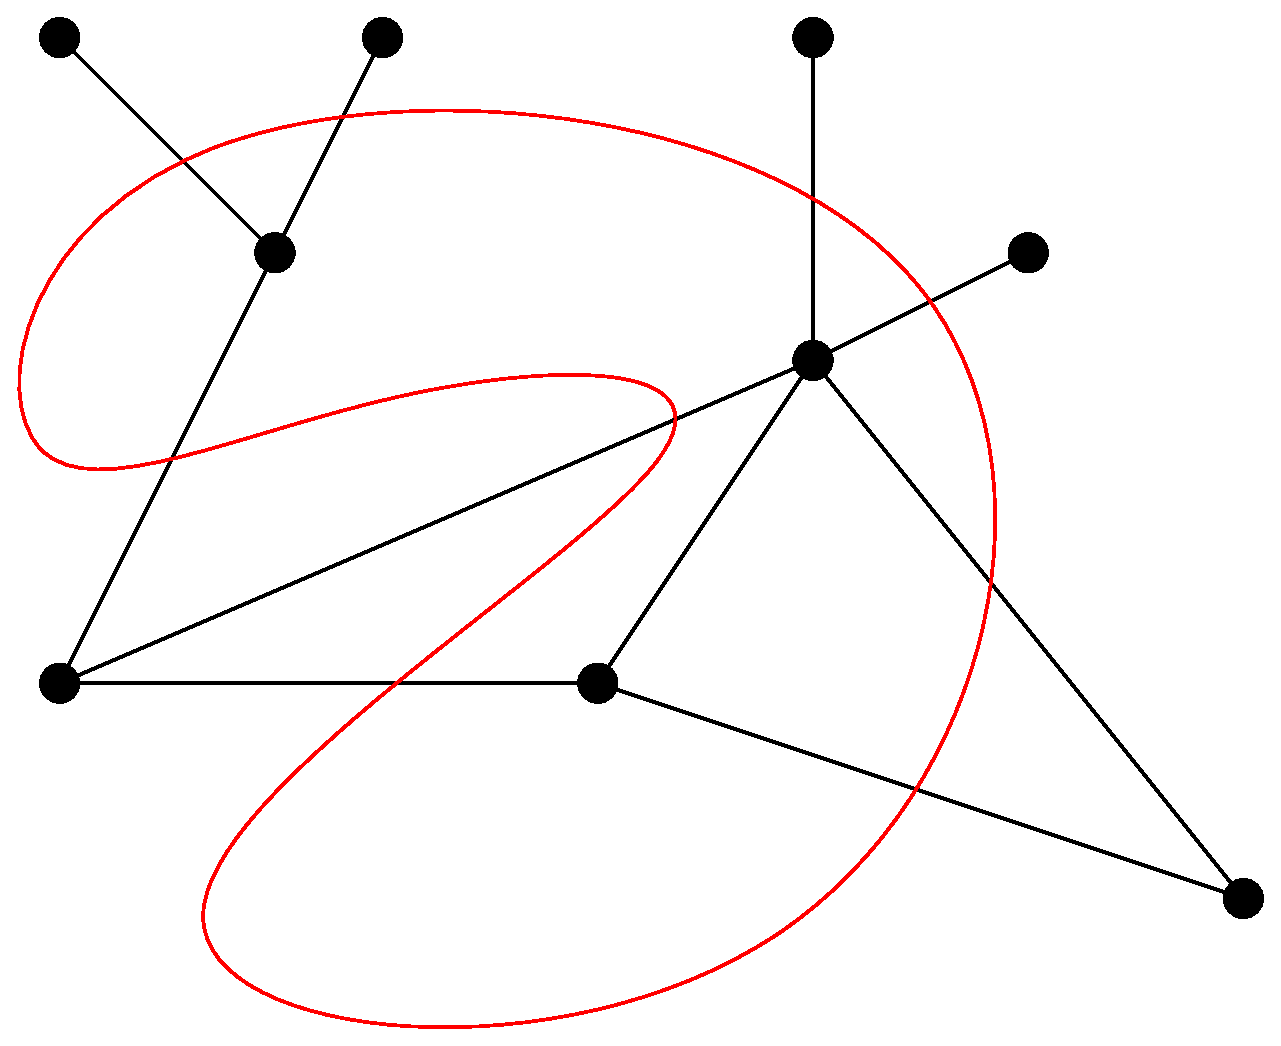
\includegraphics[width=.8\linewidth]{vc-closed.eps}}
	\end{minipage}
\end{frame}
\begin{frame} \frametitle{Planar Graphs}
	\begin{itemize}[<+->]
		\item Planar graphs are graphs\\
			\hspace{1cm}that can be \textbf{embedded} into the plane.
		\item An embedding is a crossing-free drawing.
		\item $K_5$ is not planar, but $K_4$ is.\\
			{
			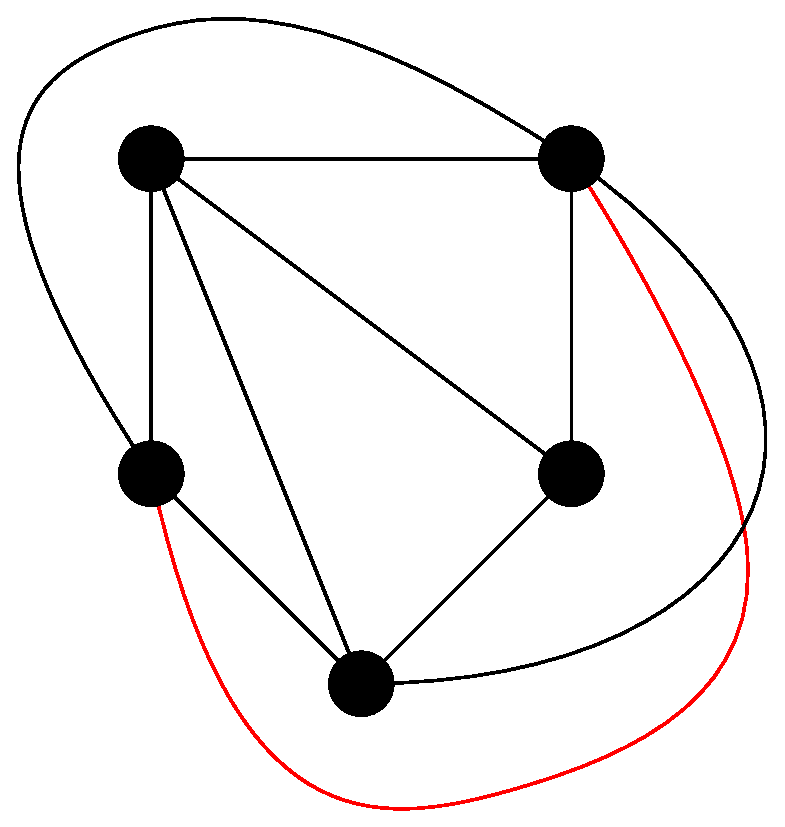
\includegraphics[width=0.3\linewidth]{k5.eps}
			\hspace{0.2\linewidth}
			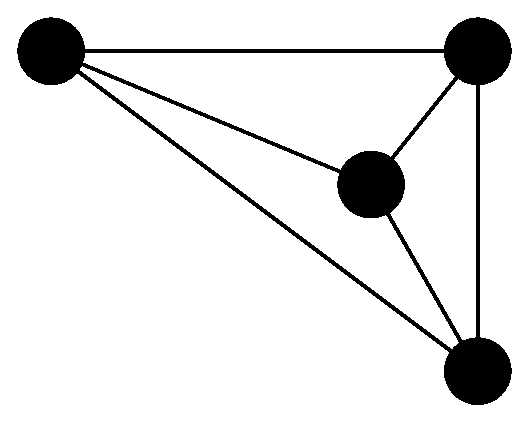
\includegraphics[width=0.3\linewidth]{k4.eps}
			}
		\item the class of planar graphs is minor-closed (why?).
			% -> we do not introduce crossings.
	\end{itemize}
\end{frame}
\begin{frame} \frametitle{Robertson and Seymour's Theorem}
	\begin{block}{Theorem 1. Robertson and Seymour's Theorem}
		The class of all graphs is well-quasi-ordered by the minor relation. That is in any
		infinite family of graphs, there are two graphs such that one is a minor of the
		other.
	\end{block}
\uncover<2->{
	\begin{block} {Corollary 2.}
		For every minor-closed graph class $\mathcal{C}$, there exists a finite set
		$\operatorname{Forb}(\mathcal{C})$ of graphs with the following property: for every
		graph $G$, the graph $G$ belongs to $\mathcal{C}$ if and only if there does not
		exist a minor of $G$ that is isomorphic to a member of
		$\operatorname{Forb}(\mathcal{C})$.
	\end{block}
}
\uncover<3->{
	\textbf{Proof sketch.}
}

\uncover<4->{
	\textbf{-Examples:}
}
\uncover<5->{
	\begin{itemize}
		\item Wagner's theorem:\\
			\hspace{.5cm}Minimal forbidden minors of planar graphs are $K_5$ and $K_{3,3}$.
		\uncover<6->{
	\item The only minimal forbidden minor of Forests is $C_3$.}
	\end{itemize}
}
	
\end{frame}
\begin{frame} \frametitle{Planarity test - a meta algorithm}
	\begin{block}{Theorem 3. Robertson and Seymour}
			There exists a computable functoin $f$ and an algorithm that, for given
			graphs $H$ and $G$, checks in time $f(H)|V(G)|^3$ whether $H \leq_m G$.
	\end{block}
	\begin{itemize}[<+->]
		\item []
		\item Theorem 3 yields an algorithm, that given a graph $G$ decides in polynomial
			time whether $G$ is planar or not.
		\item Let $\cplanar$ be the class of all planar graphs.
		\item Since $\operatorname{Forb}(\cplanar) = \{K_5, K_{3,3}\}$, it suffices to test
			the input graphs against these two minors.
		\item Using Corollary 2, we can define a similar algorithm for any minor-closed
			class of graphs.
		\item This yields an algorithm, that decides in polynomial time whether a given
			graph admits a vertex cover of size at most $k$ for a constant value of
			$k$.
	\end{itemize}
\end{frame}

\begin{frame} \frametitle{Minor-monotonousity and nonuniformly FPT}
	\begin{itemize}[<+->]
		\item We call a parameter $\rho$ minor-monotone,\\
			\hspace{1cm}if $\rho(H)\leq \rho(G)$ for all $H \leq_m G$.
		\item Vertex cover number is minor monotone. (why?)
		\item Longest path and feedback vertex number are also minor-monotone.
		\item Given a parameter $\rho$ and a constant $k$,\\
		\hspace{1cm}let $\mathcal{C}_{\rho, k} := \{G \colon \rho(G) \leq k\}$.
		\item If $\rho$ is minor-monotone, then $C_{\rho, k}$ is minor-closed.
		\item[] $\implies$ Decide in $O(f(k) n^3)$ whether a graph belongs to $C_{\rho, k}$.
		\item Not quite fixed-parameter tractable.
	\end{itemize}
\end{frame}
\begin{frame} \frametitle{Minor-monotonousity and nonuniformly FPT}
	\begin{itemize}[<+->]
		\item A problem $\mathcal{Q}$ is \textbf{nonuniformly} FPT,\\
			\hspace{1cm}if there exist
			\begin{itemize}
				\item a computable function $f:\mathbb{N}\rightarrow\mathbb{N}$,
				\item and collection of algorithms $(\mathcal{A}_k)_{k \in
					\mathbb{N}}$,
			\end{itemize}
		\item[] such that for every $k \in \mathbb{N}$ and every input $x$, 
		\begin{itemize}[<+->]
			\item the algorithm $\mathcal{A}_k$ accepts $x$ if and only if $(x,
				k)$ is a yes-instance of $\mathcal{Q}$,
			\item and $\mathcal{A}_k$ runs in time $f(k)|x|^{\alpha}$, for some constant
				$\alpha$.
		\end{itemize}
	\item For a minor-monotone parameter $\rho$,\\
		\hspace{1cm}finding $\rho(G)$ of a given graph $G$ is nonuniformly FPT.
	\end{itemize}
	
\end{frame}
\begin{frame}\frametitle{Vertex-deletion distance}
	\begin{itemize}[<+->]
		\item The class of independent sets $\mathcal{I}$ is minor-closed.
		\item Given a graph $G$. The vertex cover number of $G$
		\item[] \hspace{1cm} is the number of vertex-deletions to independent sets.
		\item Vertex cover number is vertex-deletion distance to independent sets.
		\item $G$ has vertex-deletion distance $k$ from $\mathcal{G}$,
		\item[] \hspace{1cm} if there is $S \in V, |S| \leq k$ s.t. $G \setminus S \in
			\mathcal{G}$.
		\item $\mathcal{G} + k v$ graphs with vertex-deletions distance at most $k$ to
			$\mathcal{G}$.
		\item $\mathcal{I} + k v$ is class of graphs with vertex cover number $k$.
	\end{itemize}
\end{frame}
\begin{frame}\frametitle{Vertex-deletion distance}
	\begin{itemize}[<+->]
		\item Vertex cover number $k$ is minor-closed.
		\item More generally:
		\item[] The class of graphs with vertex-deletion distance $k$\\
			to a minor-closed class of graphs is minor-closed. (why?)
		\item[]\centering 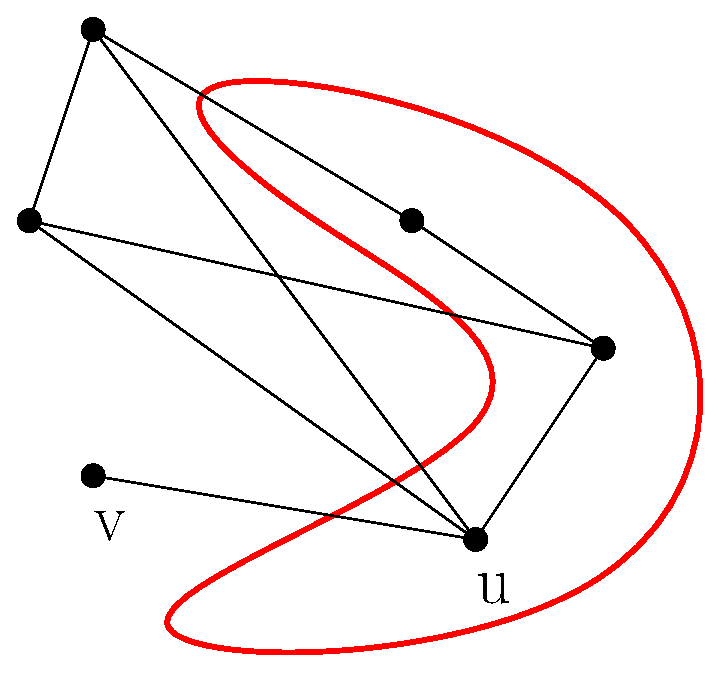
\includegraphics[width=.4\linewidth]{minor-closed.eps}
		\item Vertex-deletion distance to a minor-closed class is minor-monotone.
	\end{itemize}
\end{frame}
\begin{frame}\frametitle{Vertex-deletion distance}
	\begin{itemize}[<+->]
		\item $\mathcal{G}$ Vertex-deletion Problem:
			\begin{itemize}
				\item Given $G$ and $k$.
				\item Does $G$ have vertex-deletion distance $k$ from $\mathcal{G}$?
			\end{itemize}
		\item For each minor-closed class $\mathcal{G}$, 
		\item[] \hspace{1cm} $\mathcal{G}$ vertex-deletion problem is nonuniformly FPT.
		\item Example: Feedback vertex number is vertex-deletion distance to forests.
	\end{itemize}
	\vfill
	\vfill
	\hfill
	\uncover<7->{
	{\color{red}Thanks for listening!} \smiley}
\end{frame}
\end{document} 
